\documentclass[../main.tex]{subfiles}
\begin{document}
\section{Introduction}

Residential segregation, particularly along racial lines, is a salient and persistent feature of Western societies. Despite this, limited evidence exists of how ethnic neighborhood composition directly affects the decision to move. This likely reflects the complexity involving credible identification of the importance of neighbor identity, be it education, income or ethnicity.     

\textcite{schelling1971dynamic} remains the foundational piece in the literature on theoretical determinants of segregation. The key prediction of \textcite{schelling1971dynamic} is that neighborhoods will experience "tipping points" of different-race neighbor that elicit a "white flight" response, even for relatively mild/tolerant preferences. "Tipping behavior" has been frequently analyzed in the US (\textcite{Ananat_2011, davis2018long, chetty2015impacts}), but less so in Europe (\textcite{bohlmark_willen_2020_tipping}), let alone Denmark. 

In this paper, I aim to credibly estimate how households respond directly to receiving a new different-type neighbor.


The paper is structured as follows. 

\subsection{Definitions}
\label{sec:intro_definitions}
In the paper, I define 3 mutually exclusive types of households. (i) \textit{Native} households, where all members are of Danish origin; (ii) \textit{Non-West} households, where at least one member is of non-West origin and (iii) \textit{Western} households, where at least one household member is non-Native and has Western origin \textit{and}, but with no members that have \textit{non-Western} origin. I follow the definition of West/non-West countries by \textcite{west_non_west_def_dst}.
\end{document}







% 1) Determine treat/control
% - Treat: New non-West among K=3
% - Control: New non-west among K=4,..,40? 
% - Drop everyone else
% 2) Make panel. use lf.join_where(pl.date_range(..., eager=True)
% 3) Take unique ID's and collect
% - Inc, edu, emp
% 4) just have a little looksy @ BBR / DAR

%Section \ref{sec:model} outlines and  simulates a simplified of the Schelling model. Section \ref{sec:data} describes the data used in this paper. The empirical strategy is presented in Section \ref{sec:empirical_strategy}. The main results, including a heterogeneity analysis (?), are presented in Section \ref{sec:results}. In Section \ref{sec:Discussion}, I discuss some stuff(?). In Section \ref{sec:conclusion} I summarize and conclude.
Cont...

Include some stats:

\begin{figure}[H]
\centering
\caption{Different-type neighbors}
    \begin{subfigure}{0.47\textwidth}	
	\centering
    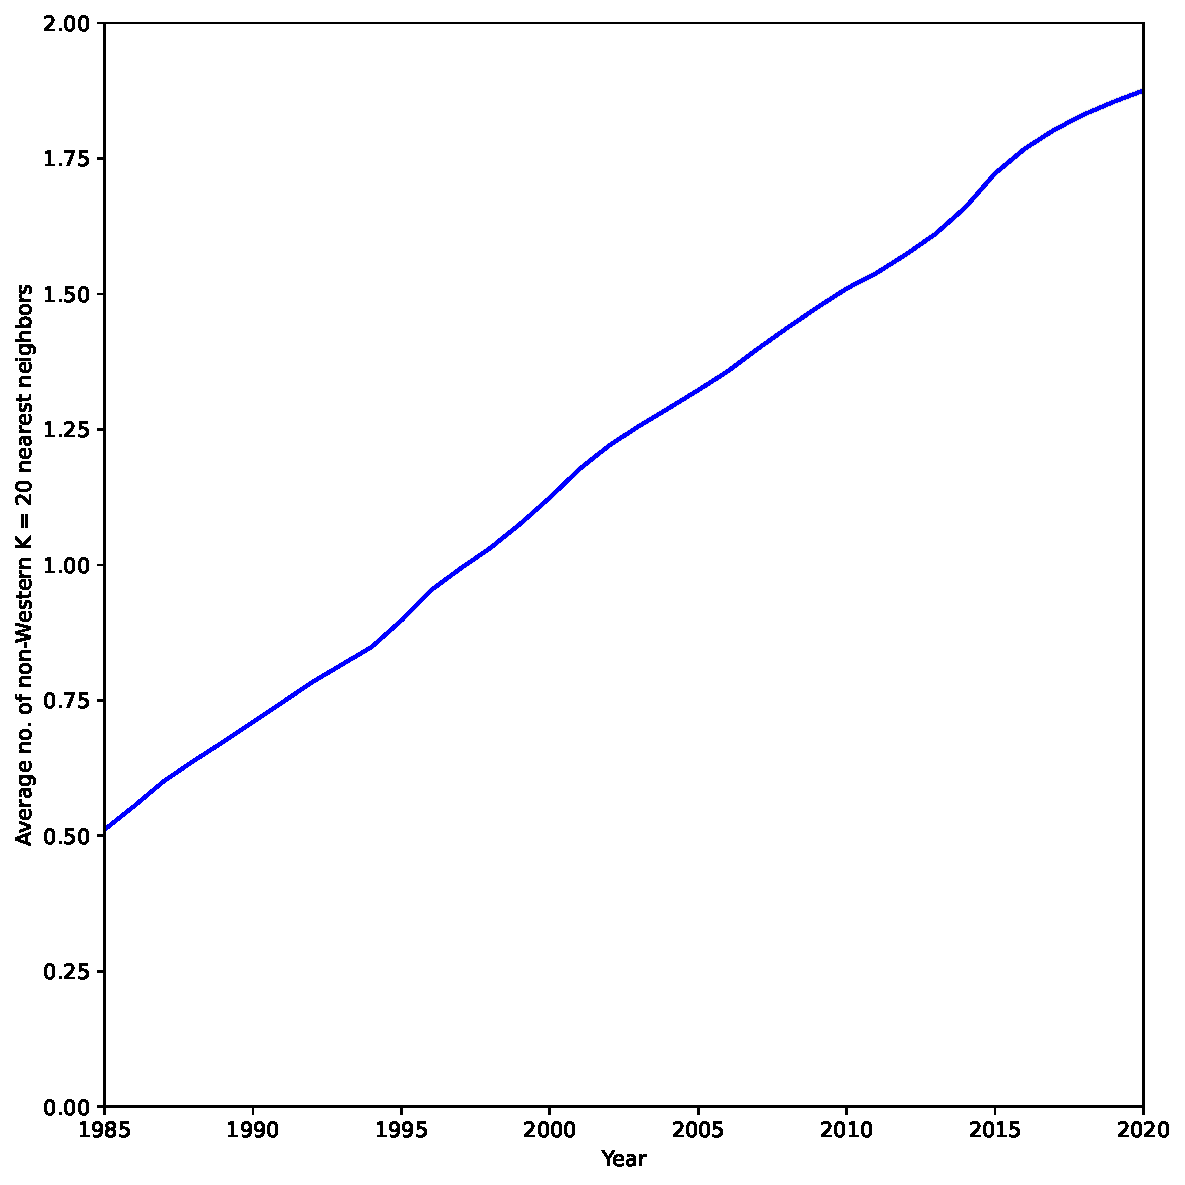
\includegraphics[width=\linewidth]{figs/mix_non_west_pos_nn_1985_2020.pdf}
	\caption{Non-Western neighbors} 
	\end{subfigure}	
    \begin{subfigure}{0.47\textwidth}	
	\centering
    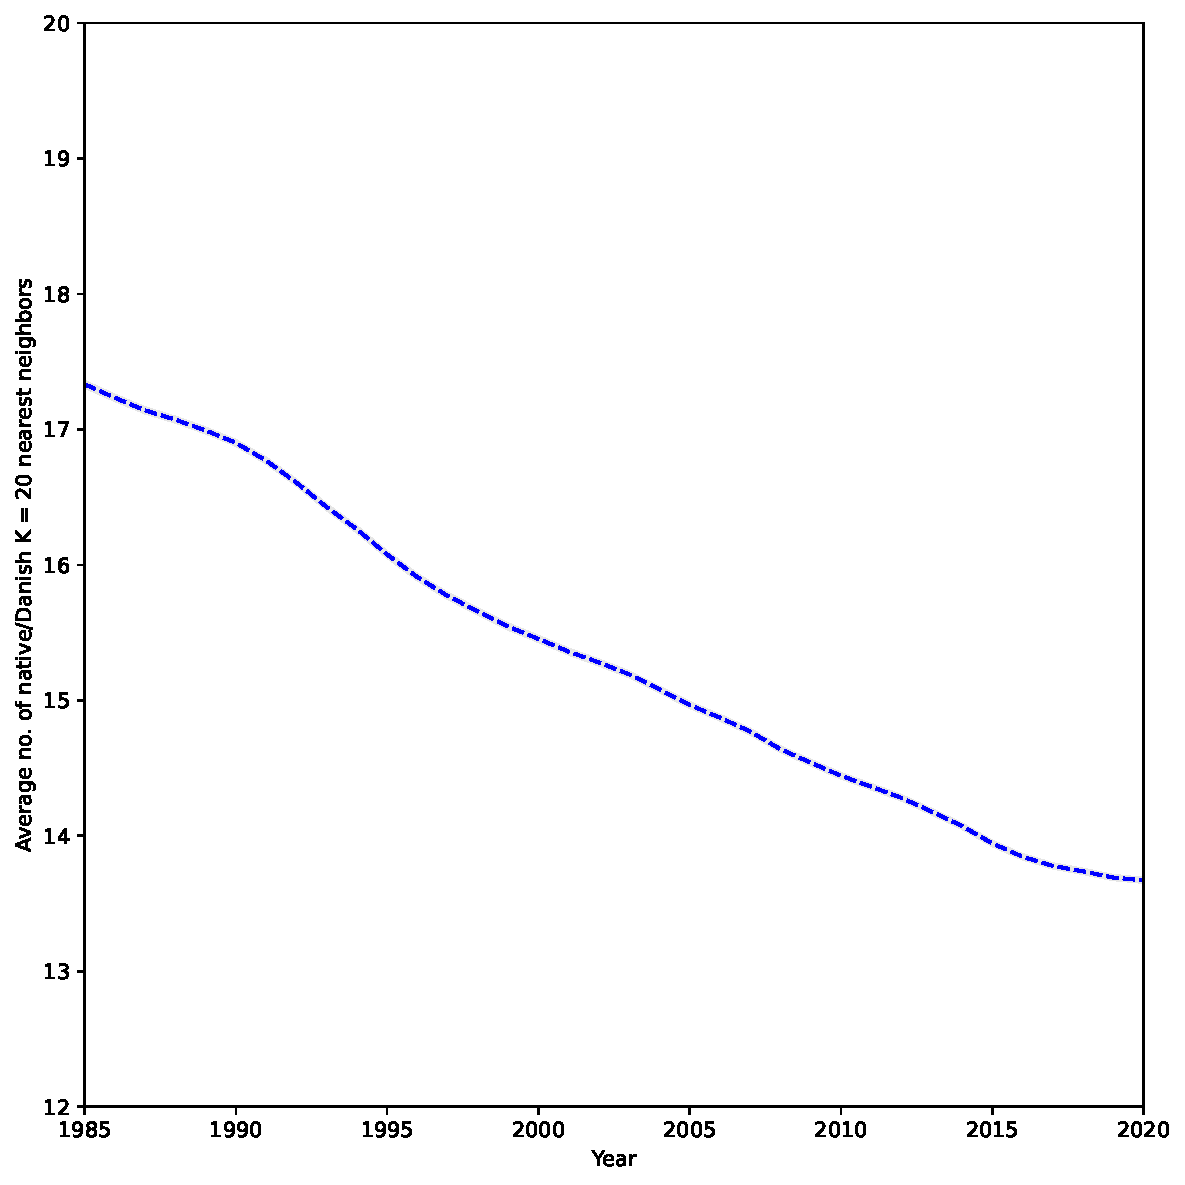
\includegraphics[width=\linewidth]{figs/native_nn_1985_2020.pdf}
	\caption{Danish/native neighbors} 
	\end{subfigure}	
      
    \label{fig:avg_k_nearest_dk}
    \begin{minipage}{.9\linewidth}
        \footnotesize \textit{Note}: Non-Western households refers to households where at least one household member is of non-Western origin. Danish/native households refers to households where all members is of Danish descent.
    \end{minipage}
\end{figure}

Some figures yet to be determined where to place can be found in Appendix \ref{sec:appendix_figs}
